\newpage

\section{Generative and Autoregressive Models}
\subsection{Generative Models}
\subsubsection{Discriminative vs Generative models}
A \emph{discriminative model} is the most common type of supervised learning model: for any input $x$, it predicts its label $y$. Probabilistically speaking, a dscriminative model learns the conditional probability distribution $\P(y|x)$, that is the probability for each label to correspond to the input. 

A \emph{generative model} learns the probability distribution $\P(x)$, or in the case of a \emph{conditional generative model}, the conditional distribution $\P(x|y)$, which present a huge mathematical and practical distinction with discriminative models.

Note that a discriminative model has no way to handle \say{unreasonable inputs}: if an input does not fit the training distribution, the model still needs to output a probability distribution over the outputs set. Nevertheless, generative models can predict the likeliness of an input to belong to the input distribution: it can \say{reject} unreasonable inputs by assigning small probabilities to them.

According to Bayes' rule, it is possible to build a conditional generative model from other components:
\begin{equation*}
    \underbrace{\P(x|y)}_{\substack{\text{Conditional}\\ \text{Generative Model}}} = \frac{\overbrace{\P(y|x)}^{\text{Discriminative Model}}}{\underbrace{\P(y)}_{\text{Prior over labels}}}\cdot\underbrace{\P(x)}_{\substack{\text{Unconditional}\\ \text{Generative Model}}}
\end{equation*}
This shows that building an unconditional generative model provides a conditional one without additional complexity.

Generative models can be used for a variety of tasks, including the detection of unlikely inputs, features learning and the generation of new input data by sampling from the learned distribution.

\subsubsection{Taxonomy of generative models}
Various types of generative models have emerged. The main distinctions can be made between models that can compute $\P(x)$ (explicit density models) and models that can only sample from it (implicit density models).
\begin{figure}[H]
    \centering
    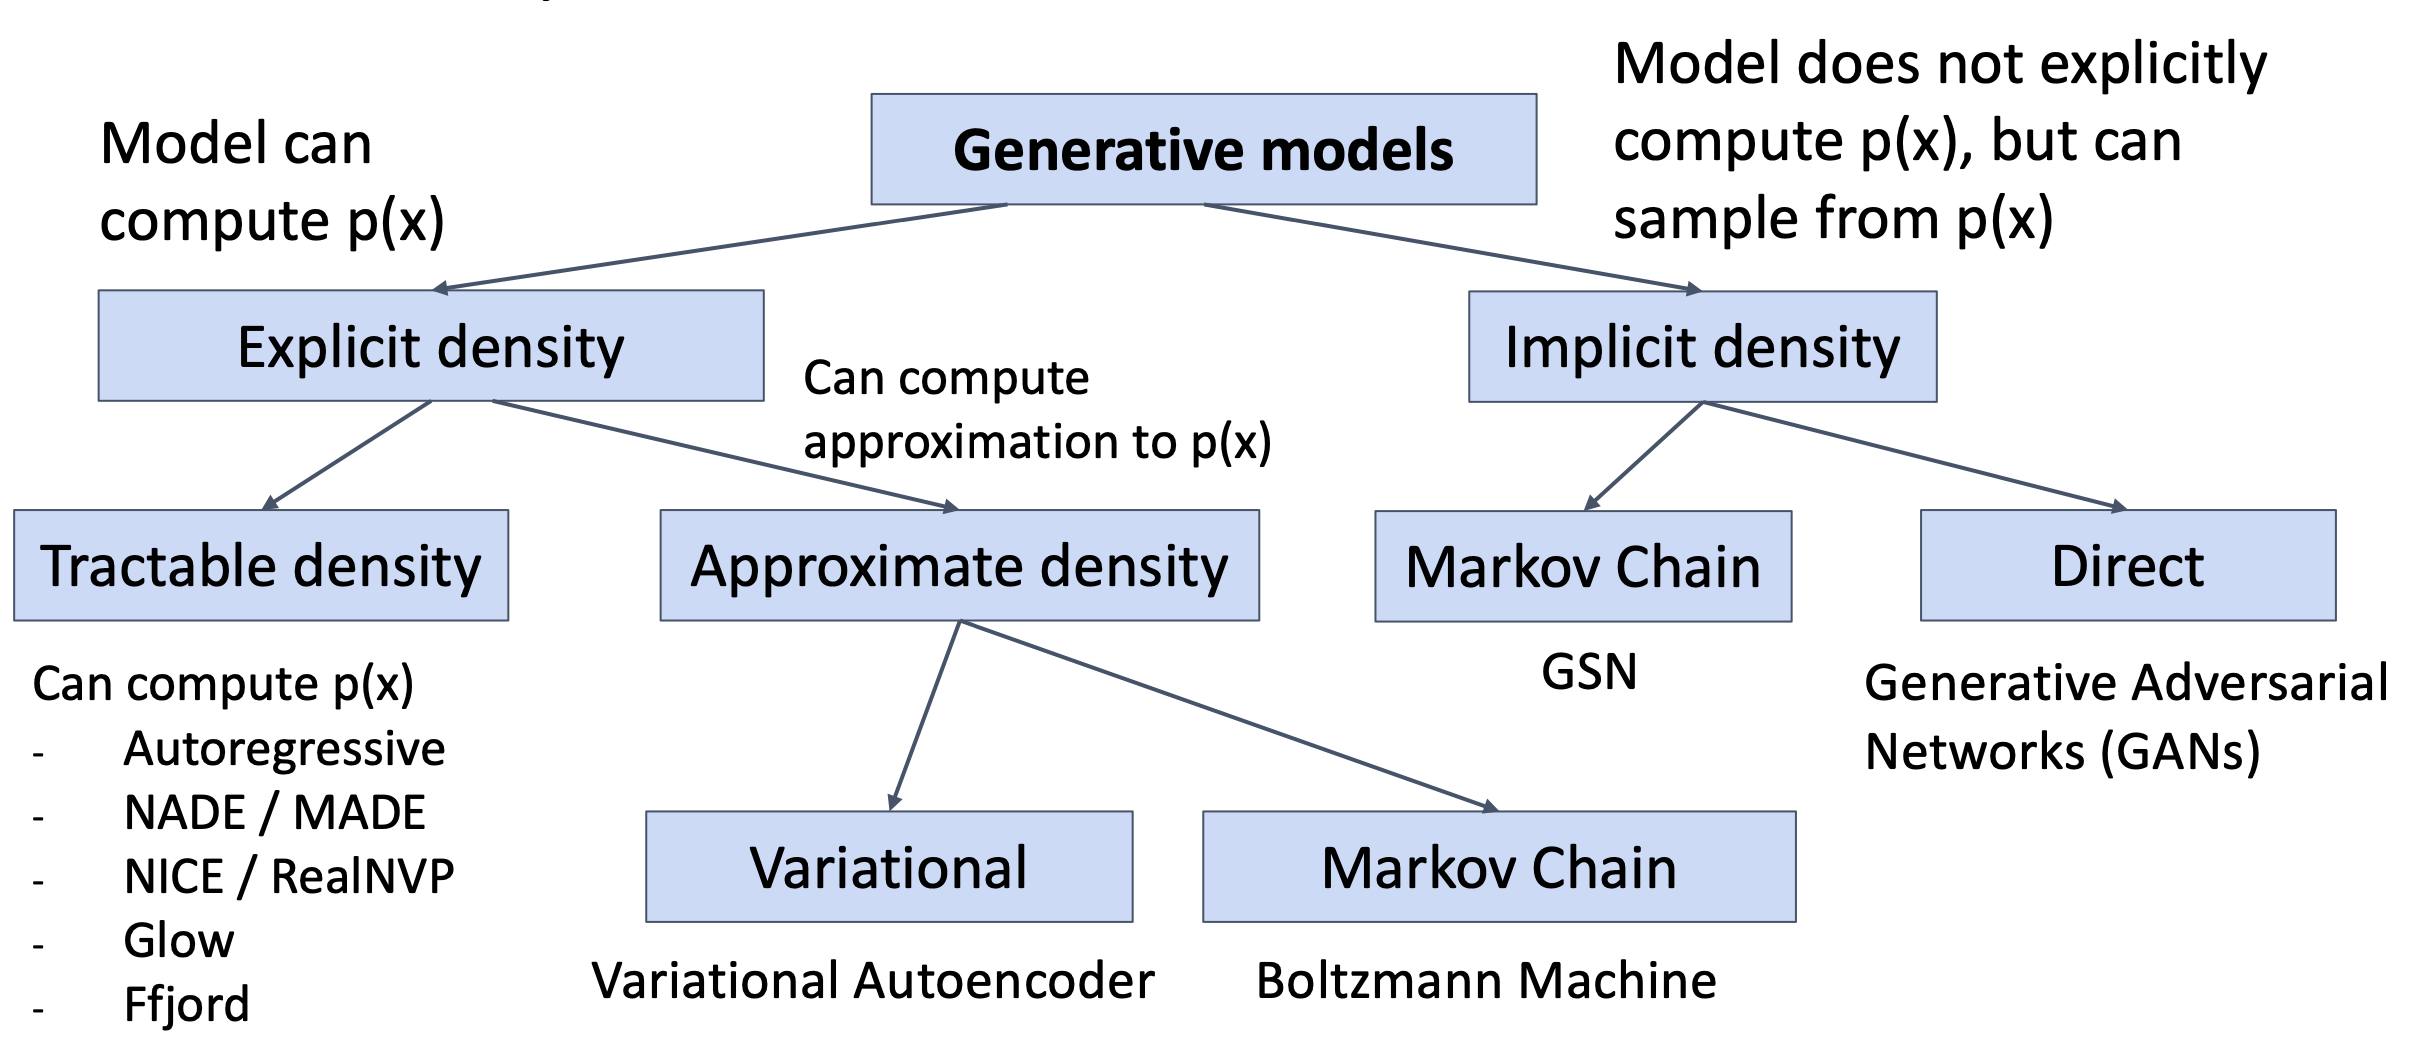
\includegraphics[width=.75\textwidth]{autoencoders/taxonomy-generative.png} 
    \caption{Taxonomy of generative models}
\end{figure}
In this chapter, we will study an explicit and tractable density model family, the autoregressive models. In the next chapters, we will introduce Variational Autoencoders and Generative Adversarial Networks. 

\subsection{Autoregressive Models}
\subsubsection{Explicit density estimation}
Our goal is to write an explicit function for the likelihood $\P(x)$, that is to find a parametric function $f_\theta$ such that for a certain learned value of $\theta^*$,
\begin{equation*}
    \forall x,\quad \P(x) = f_{\theta^*}(x)
\end{equation*}
Given a label-less dataset $(x^{(1)}, \dots, x^{(N)})$, we can train the model by solving the equation:
\begin{equation*}
    \begin{aligned}
        \theta^* &:= \argmax_\theta \prod_{i=1}^N \P(x^{(i)})\\
        &= \argmax_\theta \sum_{i=1}^N \log\P(x^{(i)})\\
        &= \argmax_\theta \sum_{i=1}^N \log f_\theta(x^{(i)})
    \end{aligned}
\end{equation*}
corresponding to maximum likelihood estimation. Therefore, we can simply take:
\begin{equation*}
    \L : \theta \longmapsto \sum_{i=1}^N \log f_\theta(x^{(i)})
\end{equation*}
as a loss function, and minimize it using gradient descent. In most practical applications, $\left(f_\theta\right)_\theta$ is a family of neural networks.

\subsubsection{Explicit density estimation using a regressive model}
The specificity of autoregressive models is to assume that each training sample $x^{(i)}$ consists of multiple subparts $(x_1^{(i)}, x_2^{(i)}, \dots, x_T^{(i)})$. For instance, in the case of images, each subpart can be a specific pixel.

We can break down the probability of observing a specific input by 

\newpage
\section{Autoencoders}
An \emph{autoencoder} is a type of neural network used to solve unsupervised learning problems. The main idea of an autoencoder is to learn an efficient representation of the input data, usually of the form of a hidden layer of size smaller than the input size. It can be useful in dimensionality reduction, but the mostly used variant is the \emph{variational autoencoder}, a certain type of generative model.

\newpage